\ctitle{Medisinsk bioteknologi}

\paragraph{Dette kapittelet} handler om virus og hvordan de fungerer, immunforsvaret, og hvordan vi kan bruke vaksiner til å sette immunforsvaret på rett kurs.

\cstitle{Virus}\index{virus}

\paragraph{Virus} Et virus er en liten genetisk enhet/agens/dingsboms som benytter seg av den reproduktive mekanismen til verten den infiserer for å reprodusere seg selv. Siden virus ikke har sin egen metabolisme, regnes de ikke som levende organismer i seg selv (de er i beste fall på grensen). Nakne virus er beskyttet av en proteinkjerne som kalles et kapsid. ``Enveloped viruses'' beskytter seg selv ved å ta med seg en bit av vertens cellemembran som et ekstra lag med beskyttelse. Noen virus koder for enzymer som de trenger for å reprodusere - blant annet har retrovirus revers-transkriptase\index{revers-transkripsjon}, som brukes for å lage DNA fra RNA. Kort sagt klarer virus å pakke inn utrolig mye sluhet i et vanvittig lite volum (de har typisk en lengde på rundt 50 nanometer).

Virus kan enten inneholde RNA eller DNA. Eksempler på RNA-virus er HIV, meslinger, rabies, tobakkmosaikkvirus, poliovirus, forkjølelse og SARS. Eksempler på DNA-virus er kopper, kukopper, herpes og bakteriofager.

\paragraph{Lytisk angrep}\index{lytisk angrep} Viruset binder seg til overflaten av cellen og injiserer det genetiske materialet. Cellens egne enzymer og ribosomer sørger for å lage mange kopier av virusets bestanddeler ved å replikere det virale genmaterialet og produsere de virale proteinene. Til slutt setter de forskjellige bestanddelene seg sammen til mange nye, hele virus, som destruerer cellen som skapte dem og sprer seg videre i miljøet (eller, hvis cellen er del av en flercellet organisme, resten av organismen). 

\paragraph{Sovende viralt DNA}\index{sovende viralt DNA} Etter å ha infiltrert verten kan viruset, i stedet for å umiddelbart reprodusere og destruere cellen, forbli inaktivt. Det virale DNAet blir replikert sammen med resten av cellen når cellen deler seg. Først senere, etter flere celledelinger, slår viruset til.

\paragraph{Ikke-lytisk angrep}\index{ikke-lytisk angrep} Viruset angriper på andre måter enn å ødelegge cellen, for eksempel når et ``enveloped virus'' tar med seg litt cellemembran. Enkelte virus kan også angripe celler ved å integrere genomet sitt i verten.

\paragraph{Antivirale medisiner}\index{antiviral medisin} Antibiotika har ingen effekt på virus, siden virus ikke har noen egen metabolisme som antibiotika kan angripe. I stedet forsøker man å tukle med hver av de forskjellige stegene i virusets reproduksjonssyklus:
\begin{itemize}[noitemsep,nolistsep]
	\item Fusjonshemmere:\index{fusjonshemmer} forhindrer viruset fra å trenge inn i cellen ved å binde seg til de samme reseptorene som viruset binder seg til når det skal trenge inn i cellen.
	\item Transkriptasehemmere:\index{transkriptasehemmer} molekyler som stikker kjepper i hjulene for reverstranskriptaseenzymet til retrovirus ved at de ligner på nukleotider, slik at enzymet feilaktig setter inn transkriptasehemmeren i polynukleotidkjeden. Dette fører til ubrukelig DNA som ikke kan leses.
	\item Integrasehemmere/antisense RNA:\index{antisense-RNA}\index{integrasehemmer} RNA som er eksakt komplementært til virusets RNA, og binder seg til det. Dermed dannes et ubrukelig RNA/RNA-hybrid som ikke kan brukes til å danne nye viruskomponenter.
	\item Proteasehemmere:\index{proteasehemmer} klipper opp de virale polypeptidene i små fragmenter akkurat når de skal settes sammen til nye virus. 
\end{itemize}

\paragraph{Naturlige strategier mot virus} Blant menneskelige cellers naturlige forsvarsmekanisme mot virus finnes inhibitorer som blokkerer reversskriptase (mot retrovirus), antistoffer (senere avsnitt), og interferoner (neste avsnitt).

\paragraph{Interferon}\index{interferon} Signalprotein som produseres av virusinfiserte celler for å si ifra til immunsystemet om at cellen er infisert og skal destrueres.

\cstitle{Immunforsvar}\index{immunforsvar}

\paragraph{Immunsystemet} Det komplekse systemet som gjør organismen i stand til å skille mellom ``selv'' og ``ikke-selv''. Immunsystemet består av den humorale immunresponsen og den cellulære immunresponsen. Man kan også dele det inn i medfødt og adaptiv immunrespons - mer om det senere.

Her er en fin video som forklarer immunsystemet: \url{https://www.youtube.com/watch?v=zQGOcOUBi6s}. En del av det som står i Renneberg nevnes også i videoen, og gjentas derfor ikke her. På samme Youtube-kanal finnes også beskrivelser av mekanismene til forskjellige virus (meslinger, HIV, ebola). \#viralvideo

\paragraph{Den humorale immunresponsen}\index{humoral immunrespons} bruker \emph{antistoffer} - proteiner som produseres av B-celler (eller mer presist: B-celler produserer plasmaceller, som produserer antistoffer) for å beskytte mot fremmede stoffer (for eksempel fra infiserende virus/bakterier) som i denne sammenhengen kalles antigener. Antistoffer binder seg til antigener på svært spesifikt vis for å markere dem som inntrengere og oppfordre makrofager til å spise dem opp.

\paragraph{Epitop}\index{epitop} Den delen av et antigen som antistoffet binder seg til. Kalles også \ix{antigendeterminant}. 

\paragraph{Strukturen til et antistoff}\index{antistoff} Antistoffer består av 4 proteinkjeder - to ``lette'' L-kjeder og to ``tunge'' H-kjeder. Proteinkjedene holdes sammen av disulfidbindinger. Disse settes sammen til en Y-form (se figur i bok/internett). Bunnen av Y-en er en ``fot'' som kalles Fc (fragment constant) som holder antistoffet til overflaten av  B-cellen. Samtidig har de en variabel region - Fv - som er antigen-spesifikk. Cellen har standardiserte polypeptidelementer som den kan bruke for å bygge molekylære antistoffer for opp til 100000000 forskjellige antigener (men man har altså ikke gener for hvert eneste antigen - det ville vært uøkonomisk).

\paragraph{Den cellulære immunresponsen}\index{cellulær immunrespons} består av \ix{T-celle}ne. Blant disse har man \idx{cytotoksiske T-celler} (``killer T-cells'') som er på utkikk etter fremmede komponenter på overflaten til cellene de møter - og hvis de finner fremmede komponenter, destruerer de cellen. Mange celler hjelper til med dette ved å kutte ut et fragment av peptider som stammer fra nedbrytningen av proteinene til en inntrenger. Dette fragmentet transporteres til overflaten av cellemembranen, der MHC-proteiner (major histocompability complex) viser frem fragmentet til omverdenen. I tillegg til cytotoksiske T-celler finnes det T-hjelpeceller som fremmer vekst av B-celler og cytotoksiske T-celler når de trengs.

\paragraph{Neopterin}\index{neopterin} En liten molekylær forbindelse som skilles ut av makrofager når de stimuleres av interferon-$\gamma$ (som skilles ut av T-hjelpeceller). Dette skjer allerede før immunsystemet har identifisert intrengeren, så å teste neopterinnivåene i blodet gir en rask test for virusinfeksjoner: en høy konsentrasjon av neopterin indikerer at det foregår et eller annet viralt angrep. Siden det skilles ut uavhengig av hvilket virus som angriper, er det spesielt nyttig for å teste bloddonorer.

\paragraph{Medfødt immunrespons}\index{medfødt immunrespons} Betegnelsen for den delen av immunresponsen som er rask, men uspesifikk. Dette er den evolusjonært eldste delen av immunsystemet, i motsetning til...

\paragraph{Adaptiv immunrespons}\index{adaptiv immunrespons} Den delen av immunresponsen som husker hvilke antigener som har vært til stede tidligere. Ved første eksponering for et patogen vil den adaptive immunresponsen være tregere - men ved senere eksponeringer vil den adaptive immunresponsen være like rask som, og mer effektiv enn, den medfødte immunresponsen, se Figur~\ref{fig:immuneresponse}. Dette fordi det da finnes ``\ix{minne-celler}'' (dette er spesialiserte T- og B-celler) som ``husker'' den første eksponeringen og ``vet'' hvordan immunsystemet må handle for å raskt og effektivt eliminere akkurat dét patogenet. Det er denne egenskapen til immunsystemet som utnyttes med vaksiner.

\begin{figure}[H]
	\centering
	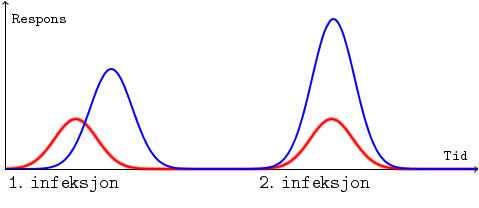
\includegraphics[width=0.50\textwidth]{immuneresponse.png}
	\caption{Skisse av immunrespons ved første og andre eksponering for et patogen. Rødt: medfødt immunrespons. Blått: adaptiv immunrespons.}
	\label{fig:immuneresponse}
\end{figure}

\cstitle{Vaksine}\index{vaksine}

\paragraph{Vaksine} Immunogent materiale som gjør at immunsystemet produserer ``minne-celler'' for en bestemt type patogen (sykdomsfremkallende virus eller mikroorganisme). Dette gjør at immunsystemet raskt kan produsere riktig type antistoffer dersom patogenet skulle angripe på et senere tidspunkt. Dermed blir man (i det ideelle tilfellet) immun mot patogenet. 

\paragraph{Den første vaksinen} var mot kopper, og ble utført ved at Edward Jenner testet sin hypotese om at det å overleve kukopper gir en livslang immunitet mot både kukopper og \ix{kopper}: han injiserte en liten dose puss fra en kukopp-infisert jente i blodet til en gutt. To uker senere injiserte han den samme gutten med en potensielt dødelig dose kopper. Gutten overlevde dette, og begynte antakelig å gruble over hva i alle dager det var han hadde gjort for at det var akkurat \emph{han} som ble valgt ut til et slikt latterlig uetisk eksperiment. Grunnen er at kukopper er nært beslektet med kopper, og de samme antistoffene som virker mot kukopper virker også mot kopper.

\paragraph{Moderne vaksiner} tar i bruk
\begin{itemize}[nolistsep,noitemsep]
	\item \ix{toksoider}: nøytraliserte ekstrakter av toksinene som patogenene skiller ut
	\item døde eller svekkede patogener som er harmløse, men fortsatt trigger en immunrespons
	\item genmodifiserte varianter av patogener, som det for tiden forskes på
\end{itemize}
Prinsippet er det samme i hvert tilfelle: kroppen produserer de riktige antistoffene \emph{før} en eventuell infeksjon.

\paragraph{Polyklonale antistoffer} Ved å immunisere et dyr mot et antigen kan man (ofte etter flere omganger med immunisering) hente ut og isolere antistoffer for antigenet fra dyret. Hvis man gjør det på denne enkleste mulige måten får man polyklonale antistoffer - en blanding av forskjellige antistoffer som alle reagerer på det samme antigenet, men som har forskjellig aminosyresekvens og binder seg til forskjellige steder (epitoper) på antigenet med forskjellig styrke.

\paragraph{Monoklonale antistoffer}\index{monoklonale antistoffer} Antistoffer med identisk molekylær struktur og spesifisitet, som stammer fra én enkelt type B-celler. Disse kan man få tak i ved å ta B-celler og fusjonere dem med tumorceller for å få en hybridcelle som er udødelig og deler seg raskt (som en kreftcelle), men også produserer de samme antistoffene som B-cella. Monoklonale antistoffer er et kraftig analytisk verktøy fordi man kan bruke dem til å oppdage små mengder av et antigen (for eksempel ved å sette en radioaktiv markør på antistoffene, slik at områder med antigenet ``lyser opp''). Dermed kan man for eksempel finne størrelsen og posisjonen til en tumor. Kombinert med annen teknologi kan man også levere medikasjon spesifikt til der antigenet befinner seg (targeted drug delivery).

\paragraph{\ix{ELISA-testen}} Står for ``enzyme-linked immunosorbent assay'' og kan brukes til å finne ut om pasienten har produsert antistoffer mot et bestemt virus - det vil si, om pasienten er infisert. Prosessen er som følger:
\begin{enumerate}[noitemsep,nolistsep]
	\item Man gror viruset og isolerer kapsidet ved at det adsorberes på en plate.
	\item Kroppsveske fra pasienten legges til på platen.
	\item Man legger til enzym-markerte monoklonale \emph{antistoffer mot pasientens antistoffer}.
	\item De monoklonale antistoffene som ikke har bundet seg, vaskes vekk. 
	\item Man legger til et substrat som er fargeløst, men som skifter farge i møte med enzymet på de monoklonale antistoffene.
\end{enumerate}
Løsningen vil bli farget hvis det er noe enzym der, som kun kan være tilfelle dersom det var noen antistoffer de monoklonale antistoffene kunne binde seg til - altså hvis pasienten har vært infisert. Ellers vil alle de monoklonale antistoffene vaskes ut, og løsningen forblir fargeløs.

\paragraph{Rekombinante antistoffer}\index{rekombinante antistoffer} Det er ofte nyttig å gjøre antistoffet er så lite som mulig. Dette har tradisjonelt blitt gjort ved å kløyve av alt annet enn den variable delen (Fv) av antistoffet. Hvis du ser på Box 5.3 ser du at en slik enkeltstående Fv-bit ikke vil være sammenhengende, og faller fra hverandre uten ekstra stabilisering. Derfor bruker man en ekstra peptidkjede for å lenke sammen de to halvdelene, for å få en scFv (Box 5.3, nederst til høyre). Tradisjonelt har dette blitt gjort med proteaser, men nu til dags lager man dem heller fra scratch med rekombinante organismer.

En fordel med rekombinante antistoffer er at det er mer etisk å lage antistoffer slik, enn det er å la dyr eller mennesker produsere antistoffene man vil ha. Det er også billigere og raskere, og ved å bruke \idx{E. coli} kan man utnytte alt man vet om bakterien i produksjonen.

% \paragraph{Rekombinante ``antistoffbibliotek''} [Øker variasjonen av antistoffer]. Antigenet injiseres i en mus, og når musen har blitt immun henter man ut miltceller og isolerer mRNA derfra. mRNAet inneholder kun eksonene, altså arvematerialet som koder for antistoff-genet. Kopi-DNA (cDNA) produseres fra mRNAet med reverstranskriptase, og så lages mange millioner kopier av dette med PCR (kapittel 10). cDNAet kuttes opp med restriksjons-endonukleaser, og [...]